\chapter{Case Study}
This chapter contains the focus of this report.

\section{High Level Synthesis}
Brief introduction to high level synthesis in general\\

What is directives?\\

How are they used?\\

Vivado HLS features are long list of optimisation directives which can be found in the XILINX Vivado High level synthesis user guide. These directives can be applied to interfaces, functions, loops, arrays and regions. 

\section{Example Problem}
\label{sec:example}
The problem chosen in this project is a least squares problem known from the world of optimisation. Least squares are used for regression by finding an estimate $\hat{x}$ that fulfils the equation $A\textbf{x} = \textbf{b}$. This is done using the following equation:
\begin{equation}
\label{leastsquares}
\hat{x} = (A^T * A)^{-1}*A^T*\textbf{b}
\end{equation}
The example is defined as:\\
A = $3 \times 3$~matrix
\[ \left( \begin{array}{ccc}
1 & 2 & 3 \\
3 & 4 & 5 \\
5 & 6 & 8 \end{array} \right)\] \\
b = $3 \times 1$~vector
\[ \left( \begin{array}{c}
4 \\
2 \\
1 \end{array} \right)\]
Solving the problem yields:\\
$\hat{x}$ = $3 \times 1$~vector
\[ \left( \begin{array}{c}
-5 \\
3 \\
1 \end{array} \right)\]

\section{HLS Implementation}
The implementation of a least squares function in HLS is done using the matrix multiplication example found in Lab 1 from the "High-Level Sythesis Flow on Zynq using Vivado" workshop\footnote{http://www.xilinx.com/support/university/vivado/vivado-workshops/Vivado-high-level-synthesis-flow-zynq.html}. The example is modified to fit the project at hand. A function for transposing a matrix is added to the solution along with a function for inverting a matrix. The inverse function is heavily inspired by a solution written by Mr. Ree at stackoverflow.com\footnote{http://stackoverflow.com/questions/983999/simple-3x3-matrix-inverse-code-c}.
The least squares function is defined as:
\begin{lstlisting}
#define MAT_A_ROWS 3
#define MAT_A_COLS 3
#define MAT_B_ROWS 3
#define MAT_B_COLS 1

typedef float mat_a_t;
typedef float result_t;

void leastSquares(mat_a_t a[MAT_A_ROWS][MAT_A_COLS],
      mat_a_t b[MAT_B_ROWS][MAT_B_COLS],
      result_t xhat[MAT_A_ROWS][MAT_B_COLS]);
\end{lstlisting}
with a being the A matrix mentioned in section \ref{sec:example}, b being the vector and xhat being $\hat{x}$. The flow through the function can be described as can be seen in figure \ref{fig:LSFunc}.
\begin{figure}[H]
\centering
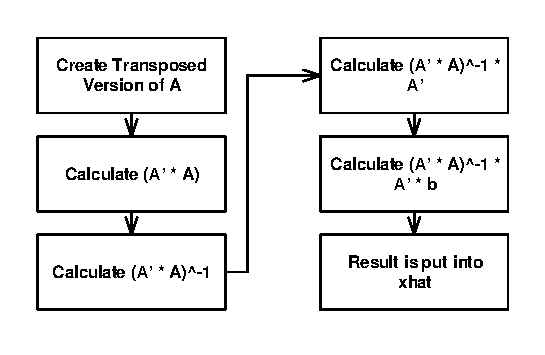
\includegraphics[scale=1]{billeder/leastSquaresFunc}
\caption{Steps in the function calculating least squares}
\label{fig:LSFunc}
\end{figure}
The testbench used in the example project has been modified in order to test the leastSquares function. The testbench is defined as:
\begin{lstlisting}
   mat_a_t in_mat_a[3][3] = {
      {1, 2, 3},
      {3, 4, 5},
      {5, 6 ,8}
   };
   mat_a_t b[3][1] = {
		   {4},
		   {2},
		   {1}
   };
   result_t hw_result[3][1];

#ifdef HW_COSIM
   // Run the AutoESL matrix multiply block
   leastSquares(in_mat_a, b, hw_result);
#endif
\end{lstlisting}
This yields the following output from the leastSquares\_csim.log file:
\begin{verbatim}
   Compiling ../../../../matrixmul_test.cpp in debug mode
   Compiling ../../../../matrixmul.cpp in debug mode
   Generating csim.exe
{
{-5}
{3}
{1}
}
@I [SIM-1] CSim done with 0 errors.
\end{verbatim}
which correspond to the solution found in section \ref{sec:example}. With the HLS Implementation complete the task is now to analyse the Sythesis.
